\documentclass[12pt]{article}
\usepackage[a4paper,margin=1.25cm]{geometry}
\usepackage{amsmath,amssymb,mathtools}
\usepackage{graphicx}
\usepackage{booktabs}
\usepackage{tabularx}
\usepackage{tikz}
\usepackage[T1]{fontenc}
\usepackage[utf8]{inputenc}
\usepackage[english]{babel}

\setlength{\parindent}{0pt}
\setlength{\parskip}{0.45em}
\setlength{\abovedisplayskip}{5pt plus 1pt minus 1pt}
\setlength{\belowdisplayskip}{5pt plus 1pt minus 1pt}
\setlength{\abovedisplayshortskip}{3pt plus 1pt minus 1pt}
\setlength{\belowdisplayshortskip}{3pt plus 1pt minus 1pt}

\newcommand{\dd}{\,\mathrm{d}}
\newcommand{\e}{\mathrm{e}}
\newcommand{\Hh}{H}

\begin{document}

\begin{center}
{\Large\bfseries A symmetric sum that is a harmonic number}\\[0.35em]
{\large the partial fraction \(\tfrac1{k(n-k)}=\tfrac1n\bigl(\tfrac1k+\tfrac1{n-k}\bigr)\) and Euler's constant}
\end{center}

\[
\boxed{\displaystyle
\lim_{n\to\infty}
\left(\frac n2\sum_{k=1}^{n-1}\frac1{k(n-k)}-\log n\right)=\gamma
=0.5772156649\ldots}
\]

\textbf{Overview.}
The sum is not merely asymptotic to a harmonic number; it \emph{equals}
one. A single partial fraction turns \(\frac{n}{2k(n-k)}\) into the
average of \(\frac1k\) and \(\frac1{n-k}\), and the reflection
\(k\mapsto n-k\) makes the two halves identical, so
\[
\frac n2\sum_{k=1}^{n-1}\frac1{k(n-k)}=\Hh_{n-1},
\qquad \Hh_m=\sum_{j=1}^{m}\frac1j .
\]
The problem then reduces to the definition of the Euler--Mascheroni
constant, \(\Hh_m-\log m\to\gamma\), with a harmless shift from \(m=n-1\)
to \(n\).

The subtraction of \(\log n\) is forced. Without it the sum diverges, and
it diverges logarithmically because \(\int_0^1\frac{\dd x}{x(1-x)}\)
diverges at both endpoints. Section 4 works this out.

\section*{1. The exact identity}

For \(1\le k\le n-1\),
\[
\frac1{k(n-k)}
=\frac{k+(n-k)}{n\,k(n-k)}
=\frac1n\left(\frac1k+\frac1{n-k}\right).
\tag{1}
\]
This is the only algebraic step. Multiplying by \(\frac n2\) and summing,
\[
\frac n2\sum_{k=1}^{n-1}\frac1{k(n-k)}
=\frac12\sum_{k=1}^{n-1}\frac1k+\frac12\sum_{k=1}^{n-1}\frac1{n-k}.
\]
The substitution \(j=n-k\) turns the second sum into the first:
\[
\sum_{k=1}^{n-1}\frac1{n-k}=\sum_{j=1}^{n-1}\frac1j=\Hh_{n-1}.
\]
Hence
\[
\boxed{\displaystyle
\frac n2\sum_{k=1}^{n-1}\frac1{k(n-k)}=\Hh_{n-1}
\quad\text{for every }n\ge2 .}
\tag{2}
\]
No approximation has been made. For instance \(n=4\) gives
\(\frac42\left(\frac13+\frac14+\frac13\right)=\frac{11}{6}=\Hh_3\).

The factor \(\frac n2\) in the statement of the problem is exactly the
normalisation that makes (2) an identity, and the symmetry
\(k\leftrightarrow n-k\) is what supplies the \(2\).

\begin{center}
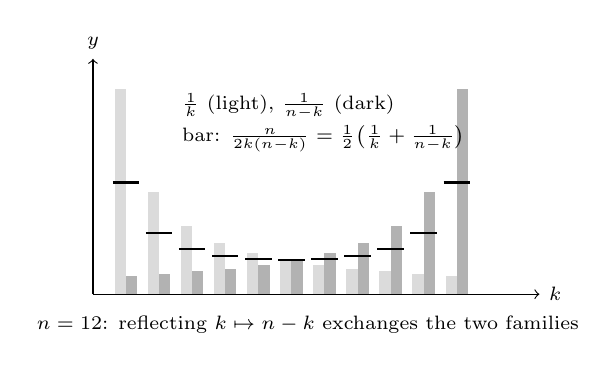
\begin{tikzpicture}[x=0.42cm,y=2.6cm]
\draw[->] (0,0)--(13.5,0) node[right] {\scriptsize \(k\)};
\draw[->] (0,0)--(0,1.15) node[above] {\scriptsize \(y\)};
\foreach \k in {1,...,11}{
  \pgfmathsetmacro{\ha}{1/\k}
  \pgfmathsetmacro{\hb}{1/(12-\k)}
  \pgfmathsetmacro{\hm}{0.5*(\ha+\hb)}
  \fill[black!14] (\k-0.34,0) rectangle (\k,\ha);
  \fill[black!30] (\k,0) rectangle (\k+0.34,\hb);
  \draw[thick] (\k-0.4,\hm)--(\k+0.4,\hm);
}
\node[anchor=west] at (2.4,0.92) {\scriptsize \(\tfrac1k\) (light), \(\tfrac1{n-k}\) (dark)};
\node[anchor=west] at (2.4,0.76) {\scriptsize bar: \(\tfrac{n}{2k(n-k)}=\tfrac12\bigl(\tfrac1k+\tfrac1{n-k}\bigr)\)};
\node[anchor=north] at (6.5,-0.06) {\scriptsize \(n=12\): reflecting \(k\mapsto n-k\) exchanges the two families};
\end{tikzpicture}
\end{center}

\section*{2. Euler's constant}

\textbf{Proposition.} The sequence \(d_m=\Hh_m-\log m\) converges.

\textit{Proof.} Compare with the integral. Since \(\frac1x\) is
decreasing, for \(j\ge1\)
\[
\frac1{j+1}\le\int_j^{j+1}\frac{\dd x}{x}\le\frac1j .
\tag{3}
\]
Summing the right inequality for \(j=1,\dots,m-1\) gives
\(\log m\le \Hh_{m-1}\), so \(d_m\ge\frac1m>0\); summing the left gives
\(\Hh_m-1\le\log m\), so \(d_m\le1\). For monotonicity,
\[
d_{m+1}-d_m=\frac1{m+1}-\log\frac{m+1}{m}
=\frac1{m+1}-\int_m^{m+1}\frac{\dd x}{x}\le0
\]
by (3). A decreasing sequence bounded below converges. \(\square\)

Its limit is by definition the Euler--Mascheroni constant,
\[
\gamma=\lim_{m\to\infty}\bigl(\Hh_m-\log m\bigr)=0.57721566490\ldots
\tag{4}
\]

\section*{3. Conclusion, with the index shift}

By (2), the quantity in the problem is \(\Hh_{n-1}-\log n\). Write it in
terms of the defining sequence:
\[
\Hh_{n-1}-\log n
=\bigl[\Hh_{n-1}-\log(n-1)\bigr]+\log\frac{n-1}{n}
=d_{n-1}+\log\left(1-\frac1n\right).
\]
The first term tends to \(\gamma\) by (4) and the second to \(\log1=0\),
so
\[
\boxed{\displaystyle
\lim_{n\to\infty}\left(\frac n2\sum_{k=1}^{n-1}\frac1{k(n-k)}-\log n\right)
=\gamma .}
\]

\textbf{Rate.} Using the standard expansion
\(\Hh_m=\log m+\gamma+\frac1{2m}-\frac1{12m^2}+O(m^{-4})\) with \(m=n\)
and \(\Hh_{n-1}=\Hh_n-\frac1n\),
\[
\Hh_{n-1}-\log n
=\gamma+\frac1{2n}-\frac1{12n^2}-\frac1n+O(n^{-4})
=\gamma-\frac1{2n}-\frac1{12n^2}+O(n^{-4}).
\tag{5}
\]
So the sequence approaches \(\gamma\) from below at rate \(\frac1{2n}\),
with the next correction \(-\frac1{12n^2}\) visible in the table below.

\begin{center}
\small
\renewcommand{\arraystretch}{1.35}
\begin{tabularx}{0.9\textwidth}{@{}lXXX@{}}
\toprule
\(n\) & \(\Hh_{n-1}-\log n\) & \(\gamma-\frac1{2n}\) & difference \\
\midrule
\(10\)    & \(0.5263832\) & \(0.5272157\) & \(-8.33\cdot10^{-4}\) \\
\(100\)   & \(0.5722073\) & \(0.5722157\) & \(-8.33\cdot10^{-6}\) \\
\(1000\)  & \(0.5767156\) & \(0.5767157\) & \(-8.33\cdot10^{-8}\) \\
\bottomrule
\end{tabularx}
\end{center}

\section*{4. Why the answer had to involve \(\gamma\)}

Rewrite the sum as a Riemann sum. With \(x_k=\frac kn\),
\[
\frac n2\sum_{k=1}^{n-1}\frac1{k(n-k)}
=\frac12\sum_{k=1}^{n-1}\frac1n\cdot\frac1{x_k(1-x_k)} .
\tag{6}
\]
The right-hand side is a Riemann sum for
\[
\frac12\int_0^1\frac{\dd x}{x(1-x)},
\]
which diverges logarithmically, and at both endpoints. That is a
diagnosis, not a failure: a divergent Riemann sum whose integrand has
simple poles at the endpoints produces a term \(\log n\) plus a constant
determined by the discrete structure, and the constant attached to
\(\frac1x\) sampled at \(\frac1n,\frac2n,\dots\) is exactly \(\gamma\).

Each endpoint contributes \(\frac12\log n+\frac12\gamma\) by (1), and the
two add up to \(\log n+\gamma\). This is the structural reason the
problem subtracts \(\log n\) rather than, say, \(\frac12\log n\), and why
the answer is \(\gamma\) rather than \(\frac\gamma2\).

\section*{5. Variants}

The same partial fraction handles a family of similar sums; the results
follow from (2) and (4) with no new ideas.

\begin{center}
\small
\renewcommand{\arraystretch}{1.5}
\begin{tabularx}{\textwidth}{@{}>{\raggedright\arraybackslash}p{0.40\textwidth}X@{}}
\toprule
Sum & Value or limit \\
\midrule
\(\displaystyle\sum_{k=1}^{n-1}\frac{1}{k(n-k)}\)
& \(\displaystyle=\frac{2\Hh_{n-1}}{n}\), exactly. \\
\addlinespace
\(\displaystyle\sum_{k=1}^{n-1}\frac{n}{k(n-k)}-2\log n\)
& \(\to 2\gamma\). \\
\addlinespace
\(\displaystyle\frac{n^2}{2}\sum_{k=1}^{n-1}\frac1{k^2(n-k)}\)
& \(\displaystyle=\frac n2\sum_{k=1}^{n-1}\left(\frac1{k^2}+\frac{1}{k(n-k)}\right)
\to\infty\) like \(\frac{\pi^2}{12}n\). \\
\addlinespace
\(\displaystyle\sum_{k=1}^{n-1}\frac1{k(n-k)}\binom{n}{k}^{-1}\)
& not reachable this way: the partial fraction (1) survives, but the
binomial weight destroys the reflection-into-itself structure of the two
halves. \\
\bottomrule
\end{tabularx}
\end{center}

The middle entry illustrates the mechanism cleanly. Applying (1) to
\(\frac{n^2}{2k^2(n-k)}\) gives \(\frac n2\left(\frac1{k^2}+\frac1{k(n-k)}\right)\);
the first part sums to \(\frac n2\cdot\frac{\pi^2}{6}+o(n)\) and dominates,
while the second contributes only \(\Hh_{n-1}=O(\log n)\). Whenever the
partial fraction produces a convergent series, that series, not the
harmonic one, sets the scale.

\end{document}
